% Options for packages loaded elsewhere
\PassOptionsToPackage{unicode}{hyperref}
\PassOptionsToPackage{hyphens}{url}
%
\documentclass[
]{article}
\usepackage{amsmath,amssymb}
\usepackage{iftex}
\ifPDFTeX
  \usepackage[T1]{fontenc}
  \usepackage[utf8]{inputenc}
  \usepackage{textcomp} % provide euro and other symbols
\else % if luatex or xetex
  \usepackage{unicode-math} % this also loads fontspec
  \defaultfontfeatures{Scale=MatchLowercase}
  \defaultfontfeatures[\rmfamily]{Ligatures=TeX,Scale=1}
\fi
\usepackage{lmodern}
\ifPDFTeX\else
  % xetex/luatex font selection
\fi
% Use upquote if available, for straight quotes in verbatim environments
\IfFileExists{upquote.sty}{\usepackage{upquote}}{}
\IfFileExists{microtype.sty}{% use microtype if available
  \usepackage[]{microtype}
  \UseMicrotypeSet[protrusion]{basicmath} % disable protrusion for tt fonts
}{}
\makeatletter
\@ifundefined{KOMAClassName}{% if non-KOMA class
  \IfFileExists{parskip.sty}{%
    \usepackage{parskip}
  }{% else
    \setlength{\parindent}{0pt}
    \setlength{\parskip}{6pt plus 2pt minus 1pt}}
}{% if KOMA class
  \KOMAoptions{parskip=half}}
\makeatother
\usepackage{xcolor}
\usepackage[margin=1in]{geometry}
\usepackage{color}
\usepackage{fancyvrb}
\newcommand{\VerbBar}{|}
\newcommand{\VERB}{\Verb[commandchars=\\\{\}]}
\DefineVerbatimEnvironment{Highlighting}{Verbatim}{commandchars=\\\{\}}
% Add ',fontsize=\small' for more characters per line
\usepackage{framed}
\definecolor{shadecolor}{RGB}{248,248,248}
\newenvironment{Shaded}{\begin{snugshade}}{\end{snugshade}}
\newcommand{\AlertTok}[1]{\textcolor[rgb]{0.94,0.16,0.16}{#1}}
\newcommand{\AnnotationTok}[1]{\textcolor[rgb]{0.56,0.35,0.01}{\textbf{\textit{#1}}}}
\newcommand{\AttributeTok}[1]{\textcolor[rgb]{0.13,0.29,0.53}{#1}}
\newcommand{\BaseNTok}[1]{\textcolor[rgb]{0.00,0.00,0.81}{#1}}
\newcommand{\BuiltInTok}[1]{#1}
\newcommand{\CharTok}[1]{\textcolor[rgb]{0.31,0.60,0.02}{#1}}
\newcommand{\CommentTok}[1]{\textcolor[rgb]{0.56,0.35,0.01}{\textit{#1}}}
\newcommand{\CommentVarTok}[1]{\textcolor[rgb]{0.56,0.35,0.01}{\textbf{\textit{#1}}}}
\newcommand{\ConstantTok}[1]{\textcolor[rgb]{0.56,0.35,0.01}{#1}}
\newcommand{\ControlFlowTok}[1]{\textcolor[rgb]{0.13,0.29,0.53}{\textbf{#1}}}
\newcommand{\DataTypeTok}[1]{\textcolor[rgb]{0.13,0.29,0.53}{#1}}
\newcommand{\DecValTok}[1]{\textcolor[rgb]{0.00,0.00,0.81}{#1}}
\newcommand{\DocumentationTok}[1]{\textcolor[rgb]{0.56,0.35,0.01}{\textbf{\textit{#1}}}}
\newcommand{\ErrorTok}[1]{\textcolor[rgb]{0.64,0.00,0.00}{\textbf{#1}}}
\newcommand{\ExtensionTok}[1]{#1}
\newcommand{\FloatTok}[1]{\textcolor[rgb]{0.00,0.00,0.81}{#1}}
\newcommand{\FunctionTok}[1]{\textcolor[rgb]{0.13,0.29,0.53}{\textbf{#1}}}
\newcommand{\ImportTok}[1]{#1}
\newcommand{\InformationTok}[1]{\textcolor[rgb]{0.56,0.35,0.01}{\textbf{\textit{#1}}}}
\newcommand{\KeywordTok}[1]{\textcolor[rgb]{0.13,0.29,0.53}{\textbf{#1}}}
\newcommand{\NormalTok}[1]{#1}
\newcommand{\OperatorTok}[1]{\textcolor[rgb]{0.81,0.36,0.00}{\textbf{#1}}}
\newcommand{\OtherTok}[1]{\textcolor[rgb]{0.56,0.35,0.01}{#1}}
\newcommand{\PreprocessorTok}[1]{\textcolor[rgb]{0.56,0.35,0.01}{\textit{#1}}}
\newcommand{\RegionMarkerTok}[1]{#1}
\newcommand{\SpecialCharTok}[1]{\textcolor[rgb]{0.81,0.36,0.00}{\textbf{#1}}}
\newcommand{\SpecialStringTok}[1]{\textcolor[rgb]{0.31,0.60,0.02}{#1}}
\newcommand{\StringTok}[1]{\textcolor[rgb]{0.31,0.60,0.02}{#1}}
\newcommand{\VariableTok}[1]{\textcolor[rgb]{0.00,0.00,0.00}{#1}}
\newcommand{\VerbatimStringTok}[1]{\textcolor[rgb]{0.31,0.60,0.02}{#1}}
\newcommand{\WarningTok}[1]{\textcolor[rgb]{0.56,0.35,0.01}{\textbf{\textit{#1}}}}
\usepackage{graphicx}
\makeatletter
\def\maxwidth{\ifdim\Gin@nat@width>\linewidth\linewidth\else\Gin@nat@width\fi}
\def\maxheight{\ifdim\Gin@nat@height>\textheight\textheight\else\Gin@nat@height\fi}
\makeatother
% Scale images if necessary, so that they will not overflow the page
% margins by default, and it is still possible to overwrite the defaults
% using explicit options in \includegraphics[width, height, ...]{}
\setkeys{Gin}{width=\maxwidth,height=\maxheight,keepaspectratio}
% Set default figure placement to htbp
\makeatletter
\def\fps@figure{htbp}
\makeatother
\setlength{\emergencystretch}{3em} % prevent overfull lines
\providecommand{\tightlist}{%
  \setlength{\itemsep}{0pt}\setlength{\parskip}{0pt}}
\setcounter{secnumdepth}{-\maxdimen} % remove section numbering
\ifLuaTeX
  \usepackage{selnolig}  % disable illegal ligatures
\fi
\IfFileExists{bookmark.sty}{\usepackage{bookmark}}{\usepackage{hyperref}}
\IfFileExists{xurl.sty}{\usepackage{xurl}}{} % add URL line breaks if available
\urlstyle{same}
\hypersetup{
  pdftitle={Tarea 2 Estadística Actuarial II},
  pdfauthor={Maria Carolina Navarro Monge C05513; Tábata Picado Carmona C05961; Jose Pablo Trejos Conejo C07862},
  hidelinks,
  pdfcreator={LaTeX via pandoc}}

\title{Tarea 2 Estadística Actuarial II}
\author{Maria Carolina Navarro Monge C05513 \and Tábata Picado Carmona
C05961 \and Jose Pablo Trejos Conejo C07862}
\date{}

\begin{document}
\maketitle

Primeramente, se cargan las librerías necesarias.

\begin{Shaded}
\begin{Highlighting}[]
\FunctionTok{library}\NormalTok{(tidyverse)}
\end{Highlighting}
\end{Shaded}

\begin{verbatim}
## Warning: package 'tidyverse' was built under R version 4.3.1
\end{verbatim}

\begin{verbatim}
## Warning: package 'ggplot2' was built under R version 4.3.1
\end{verbatim}

\begin{Shaded}
\begin{Highlighting}[]
\FunctionTok{library}\NormalTok{(readxl)}
\end{Highlighting}
\end{Shaded}

\begin{verbatim}
## Warning: package 'readxl' was built under R version 4.3.1
\end{verbatim}

\hypertarget{ejercicio-2}{%
\section{Ejercicio 2}\label{ejercicio-2}}

\textbf{Usando la metodología de Muestreo por Importancia, Si
X\textasciitilde N(0.5,0.5) estime:}

\hypertarget{a.-px-5}{%
\subsection{a. P(X\textless-5)}\label{a.-px-5}}

Primeramenre, mediante el metódo de integración por Montecarlo se
obtiene el siguiente resultado:

\begin{Shaded}
\begin{Highlighting}[]
\CommentTok{\#{-}{-}Estimación de función de distribución mediante integración por Montecarlo{-}{-}}

\FunctionTok{set.seed}\NormalTok{(}\DecValTok{2901}\NormalTok{)}
\NormalTok{n }\OtherTok{\textless{}{-}} \DecValTok{10}\SpecialCharTok{\^{}}\DecValTok{4} \CommentTok{\#tamaño de la muestra}

\NormalTok{X }\OtherTok{\textless{}{-}} \FunctionTok{rnorm}\NormalTok{(n, }\FloatTok{0.5}\NormalTok{, }\FunctionTok{sqrt}\NormalTok{(}\FloatTok{0.5}\NormalTok{))}

\NormalTok{f }\OtherTok{\textless{}{-}} \FunctionTok{dnorm}\NormalTok{(X, }\FloatTok{0.5}\NormalTok{, }\FunctionTok{sqrt}\NormalTok{(}\FloatTok{0.5}\NormalTok{))}

\NormalTok{valor\_estimado\_1 }\OtherTok{\textless{}{-}} \FunctionTok{mean}\NormalTok{(f)}

\NormalTok{valor\_real }\OtherTok{\textless{}{-}} \FunctionTok{pnorm}\NormalTok{(}\SpecialCharTok{{-}}\DecValTok{5}\NormalTok{, }\FloatTok{0.5}\NormalTok{, }\FunctionTok{sqrt}\NormalTok{(}\FloatTok{0.5}\NormalTok{))}

\NormalTok{comparacion }\OtherTok{\textless{}{-}} \FunctionTok{data.frame}\NormalTok{(}\StringTok{"Estimación"} \OtherTok{=}\NormalTok{ valor\_estimado\_1, }\StringTok{"Valor real"} \OtherTok{=}\NormalTok{ valor\_real)}

\FunctionTok{print}\NormalTok{(comparacion)}
\end{Highlighting}
\end{Shaded}

\begin{verbatim}
##   Estimación   Valor.real
## 1  0.3991698 3.678924e-15
\end{verbatim}

Como se puede observar, la estimación resultante converge lento al valor
real. Por lo tanto, mediante Muestreo por Importancia se puede acelelar
la convergencia empleando una densidad auxiliar. Para este caso, la
densidad auxiliar a utilizar es una exponencial truncada de la forma
\(\lambda e^{-\lambda(x-t)}\), con x\textgreater t.

La probabilidad a estimar es equivalente a P(X\textgreater6). Nos
basaremos en esta para aproximarla mediante el Muestro por Importancia
por medio de una exponencial truncada en 6 con \(\lambda = 1\). El
procedimiento se muestra en el siguiente algoritmo:

\begin{Shaded}
\begin{Highlighting}[]
\CommentTok{\#{-}{-}Estimación de función de distribución mediante Muestreo por Importancia{-}{-}}

\NormalTok{A }\OtherTok{\textless{}{-}} \FunctionTok{rexp}\NormalTok{(n)}\SpecialCharTok{+}\DecValTok{6} \CommentTok{\#datos aleatorios mayores a 6 con distribución exponencial}

\NormalTok{w }\OtherTok{\textless{}{-}} \FunctionTok{dnorm}\NormalTok{(A, }\FloatTok{0.5}\NormalTok{, }\FunctionTok{sqrt}\NormalTok{(}\FloatTok{0.5}\NormalTok{)) }\SpecialCharTok{/} \FunctionTok{dexp}\NormalTok{(A}\DecValTok{{-}6}\NormalTok{)}

\NormalTok{valor\_estimado }\OtherTok{\textless{}{-}} \FunctionTok{mean}\NormalTok{(w)}

\NormalTok{resumen }\OtherTok{\textless{}{-}} \FunctionTok{data.frame}\NormalTok{(}\StringTok{"Estimación"} \OtherTok{=}\NormalTok{ valor\_estimado, }\StringTok{"Valor real"} \OtherTok{=}\NormalTok{ valor\_real)}

\FunctionTok{print}\NormalTok{(resumen)}
\end{Highlighting}
\end{Shaded}

\begin{verbatim}
##     Estimación   Valor.real
## 1 3.669418e-15 3.678924e-15
\end{verbatim}

De tal manera, se obtiene una mejor aproximación de la probabilidad
P(X\textless-5), pues, es muy similar al valor real.

\hypertarget{b.-estime-el-error-absoluto-de-la-estimaciuxf3n-del-punto-a.}{%
\subsection{b. Estime el error absoluto de la estimación del punto
a.}\label{b.-estime-el-error-absoluto-de-la-estimaciuxf3n-del-punto-a.}}

El error absoluto de la estimación es:

\begin{Shaded}
\begin{Highlighting}[]
\NormalTok{error\_absoluto }\OtherTok{\textless{}{-}} \FunctionTok{abs}\NormalTok{(valor\_estimado}\SpecialCharTok{{-}}\NormalTok{valor\_real)}
\end{Highlighting}
\end{Shaded}

\hypertarget{ejercicio-4}{%
\section{Ejercicio 4}\label{ejercicio-4}}

\textbf{Sea \(f(x) = sen\left(x + \frac{cos(10x)}{3}\right)\) para
\(x\in[-2,2]\)} \#\# a.Utilizando el algoritmo de recalentamiento
simulado estime el mínimo global en {[}−2,2{]}, con valor inicial en
1.5.

Primero definimos la función en R y la graficamos para darnos una idea
de dónde puede estar ubicado el mínimo global de la función en el
intervalo.

\begin{Shaded}
\begin{Highlighting}[]
\NormalTok{fx }\OtherTok{\textless{}{-}} \ControlFlowTok{function}\NormalTok{(x)\{}\FunctionTok{sin}\NormalTok{(x }\SpecialCharTok{+}\NormalTok{ (}\FunctionTok{cos}\NormalTok{(}\DecValTok{10}\SpecialCharTok{*}\NormalTok{x)}\SpecialCharTok{/}\DecValTok{3}\NormalTok{))\} }
\FunctionTok{curve}\NormalTok{(fx,}\AttributeTok{col=}\StringTok{"violet"}\NormalTok{,}\AttributeTok{lwd=}\DecValTok{2}\NormalTok{,}\AttributeTok{from=}\SpecialCharTok{{-}}\DecValTok{2}\NormalTok{,}\AttributeTok{to =} \DecValTok{2}\NormalTok{,}\AttributeTok{n=}\DecValTok{1000}\NormalTok{,}\AttributeTok{ylab=}\StringTok{"f(x)"}\NormalTok{)}
\FunctionTok{title}\NormalTok{(}\StringTok{"Gráfico de la función"}\NormalTok{)}
\end{Highlighting}
\end{Shaded}

\includegraphics{Rmarkdown_files/figure-latex/unnamed-chunk-5-1.pdf}

Ahora definimos la función que va a ejecutar el algoritmo de
recalentamiento simulado la cual va a recibir la función definida
anteriormente, el alpha que en este caso se establece en 0.1, el valor
inicial en 1.5, número de iteraciones que para este ejercicio es de 1000
y por último, el mínimo y máximo del intervalo observado -2 y 2
respectivamente.

\begin{Shaded}
\begin{Highlighting}[]
\NormalTok{recalentamiento\_simulado }\OtherTok{\textless{}{-}} \ControlFlowTok{function}\NormalTok{(f,}\AttributeTok{alpha=}\FloatTok{0.5}\NormalTok{,}\AttributeTok{s0=}\DecValTok{0}\NormalTok{,niter,}\AttributeTok{mini=}\SpecialCharTok{{-}}\ConstantTok{Inf}\NormalTok{,}\AttributeTok{maxi=}\ConstantTok{Inf}\NormalTok{)\{ }
\NormalTok{  s\_n }\OtherTok{\textless{}{-}}\NormalTok{ s0 }
\NormalTok{  estados }\OtherTok{\textless{}{-}} \FunctionTok{rep}\NormalTok{(}\DecValTok{0}\NormalTok{,niter) }
\NormalTok{  iter\_count }\OtherTok{\textless{}{-}} \DecValTok{0} 
  
  \ControlFlowTok{for}\NormalTok{(k }\ControlFlowTok{in} \DecValTok{1}\SpecialCharTok{:}\NormalTok{niter)\{ }
\NormalTok{    estados[k]}\OtherTok{\textless{}{-}}\NormalTok{s\_n }
\NormalTok{    T }\OtherTok{\textless{}{-}}\NormalTok{ (}\DecValTok{1}\SpecialCharTok{{-}}\NormalTok{alpha)}\SpecialCharTok{\^{}}\NormalTok{k}
\NormalTok{    s\_new }\OtherTok{\textless{}{-}} \FunctionTok{rnorm}\NormalTok{(}\DecValTok{1}\NormalTok{,s\_n,}\DecValTok{1}\NormalTok{)}
    
    \ControlFlowTok{if}\NormalTok{(s\_new}\SpecialCharTok{\textless{}}\NormalTok{mini)\{}
\NormalTok{      s\_new }\OtherTok{\textless{}{-}}\NormalTok{ mini}
\NormalTok{    \} }
    
    \ControlFlowTok{if}\NormalTok{(s\_new}\SpecialCharTok{\textgreater{}}\NormalTok{maxi)\{}
\NormalTok{      s\_new }\OtherTok{\textless{}{-}}\NormalTok{ maxi}
\NormalTok{    \} }
    
\NormalTok{    dif }\OtherTok{\textless{}{-}} \FunctionTok{f}\NormalTok{(s\_new)}\SpecialCharTok{{-}}\FunctionTok{f}\NormalTok{(s\_n)}
    
    \ControlFlowTok{if}\NormalTok{(dif}\SpecialCharTok{\textless{}} \DecValTok{0}\NormalTok{)\{ }
\NormalTok{      s\_n }\OtherTok{\textless{}{-}}\NormalTok{ s\_new }
\NormalTok{    \} }\ControlFlowTok{else}\NormalTok{ \{ }
\NormalTok{        random }\OtherTok{\textless{}{-}} \FunctionTok{runif}\NormalTok{(}\DecValTok{1}\NormalTok{,}\DecValTok{0}\NormalTok{,}\DecValTok{1}\NormalTok{) }
        
        \ControlFlowTok{if}\NormalTok{(random }\SpecialCharTok{\textless{}}\FunctionTok{exp}\NormalTok{(}\SpecialCharTok{{-}}\NormalTok{dif}\SpecialCharTok{/}\NormalTok{T))\{ }
\NormalTok{          s\_n }\OtherTok{\textless{}{-}}\NormalTok{ s\_new }
\NormalTok{        \} }
        
\NormalTok{    \} }
    
\NormalTok{    iter\_count }\OtherTok{\textless{}{-}}\NormalTok{ iter\_count }\SpecialCharTok{+}\DecValTok{1}
    
\NormalTok{  \}}
  
  \FunctionTok{return}\NormalTok{(}\FunctionTok{list}\NormalTok{(}\AttributeTok{r=}\NormalTok{s\_n,}\AttributeTok{e=}\NormalTok{estados)) }
\NormalTok{\}}

\NormalTok{Resultado }\OtherTok{\textless{}{-}} \FunctionTok{recalentamiento\_simulado}\NormalTok{(fx,}\FloatTok{0.1}\NormalTok{,}\FloatTok{1.5}\NormalTok{,}\DecValTok{1000}\NormalTok{,}\SpecialCharTok{{-}}\DecValTok{2}\NormalTok{,}\DecValTok{2}\NormalTok{) }
\NormalTok{Resultado}\SpecialCharTok{$}\NormalTok{r}
\end{Highlighting}
\end{Shaded}

\begin{verbatim}
## [1] -1.806134
\end{verbatim}

Una vez ejecutado el código arroja que el mínimo global de la función es
-1.805683, para corrobar este resultado se decide graficar de nuevo la
función junto con el mínimo.

\begin{Shaded}
\begin{Highlighting}[]
\FunctionTok{curve}\NormalTok{(fx,}\AttributeTok{col=}\StringTok{"\#FFB6C1"}\NormalTok{,}\AttributeTok{lwd=}\DecValTok{2}\NormalTok{,}\AttributeTok{from=}\SpecialCharTok{{-}}\DecValTok{2}\NormalTok{,}\AttributeTok{to =} \DecValTok{2}\NormalTok{,}\AttributeTok{n=}\DecValTok{1000}\NormalTok{,}\AttributeTok{ylab=}\StringTok{"f(x)"}\NormalTok{)}
\FunctionTok{title}\NormalTok{(}\StringTok{"Gráfico y mínimo global de la función"}\NormalTok{)}
\FunctionTok{abline}\NormalTok{(}\AttributeTok{v=}\NormalTok{Resultado}\SpecialCharTok{$}\NormalTok{r,}\AttributeTok{col=}\StringTok{"\#98FB98"}\NormalTok{)}
\FunctionTok{text}\NormalTok{(Resultado}\SpecialCharTok{$}\NormalTok{r, }\DecValTok{0}\NormalTok{, }\StringTok{"Mínimo"}\NormalTok{, }\AttributeTok{pos =} \DecValTok{1}\NormalTok{, }\AttributeTok{col =} \StringTok{"\#98FB98"}\NormalTok{)}
\end{Highlighting}
\end{Shaded}

\includegraphics{Rmarkdown_files/figure-latex/unnamed-chunk-7-1.pdf}

\hypertarget{b.grafique-el-resultado-de-los-estados-donde-estuvo-la-cadena-de-la-estimaciuxf3n-del-punto-a.}{%
\subsection{b.Grafique el resultado de los estados donde estuvo la
cadena de la estimación del punto
a.**}\label{b.grafique-el-resultado-de-los-estados-donde-estuvo-la-cadena-de-la-estimaciuxf3n-del-punto-a.}}

\begin{Shaded}
\begin{Highlighting}[]
\FunctionTok{plot}\NormalTok{(Resultado}\SpecialCharTok{$}\NormalTok{e, }\AttributeTok{xlab =} \StringTok{"Iteraciones"}\NormalTok{, }\AttributeTok{ylab =} \StringTok{"Valor (x)"}\NormalTok{, }
     \AttributeTok{main =} \StringTok{"Estados de la cadena"}\NormalTok{)}
\end{Highlighting}
\end{Shaded}

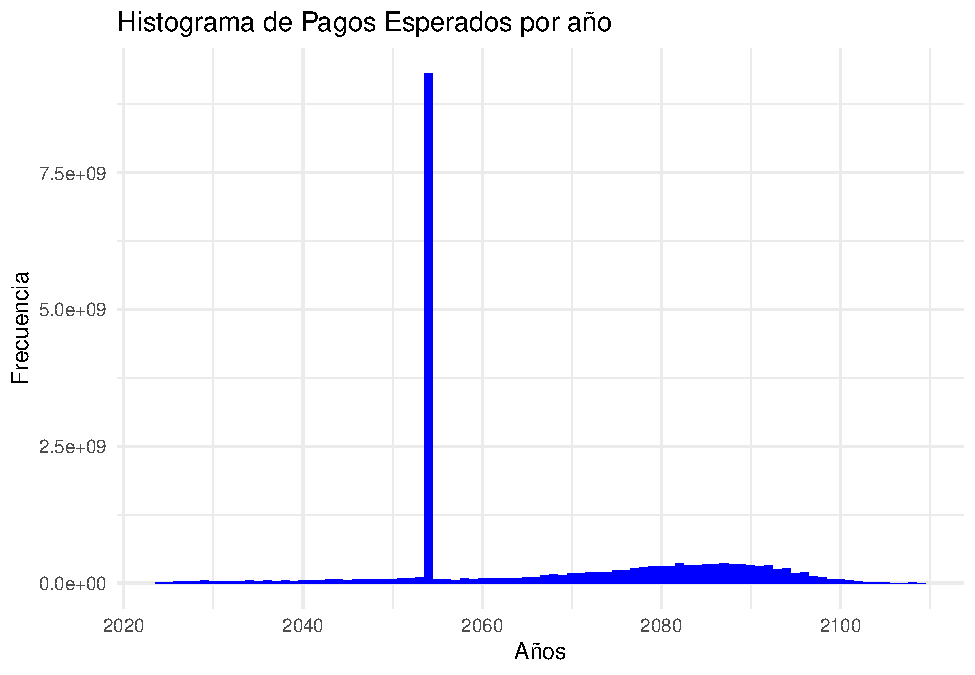
\includegraphics{Rmarkdown_files/figure-latex/unnamed-chunk-8-1.pdf}

\hypertarget{ejercicio-5}{%
\section{Ejercicio 5}\label{ejercicio-5}}

\textbf{Una aseguradora tiene un producto llamado Doble Seguro de Vida
(DSV) el cual paga 2 veces la suma asegurada si la persona fallece antes
de los 60 años, paga 1 suma asegurada cuando la persona cumple los 60
años (si no ha fallecido) y paga 1 suma asegurada si fallece después de
los 60 años. Considerando:}

\textbf{a. Las tablas de vida dinámicas de la SUPEN
(\url{https://webapps.supen.fi.cr/tablasVida/Recursos/documentos/tavid2000-2150.xls})}

\textbf{b. Un cliente de 30 años, hombre con una suma asegurable de 1
000 000 colones.}

\textbf{Construya con la ayuda de un MCMC la distribución de los pagos
por año de que se espera de este seguro. Use al menos 10 000
iteraciones. Y muestre Histograma.}

Primeramente, se carga la tabla de vida dinámica de la SUPEN y se filtra
para obtener los datos correspondientes para un hombre que en el
presente año (2024) tiene 30 años

\begin{Shaded}
\begin{Highlighting}[]
\CommentTok{\#Se carga la base de datos}
\NormalTok{tabla\_vida }\OtherTok{\textless{}{-}} \FunctionTok{read\_excel}\NormalTok{(}\StringTok{"tavid2000{-}2150.xls"}\NormalTok{,}
                         \AttributeTok{col\_types =} \StringTok{"numeric"}\NormalTok{)}

\CommentTok{\#Se filtra la base de datos para obtener los datos de un hombre nacido en 1994 }
\CommentTok{\#con edades mayor o igual a 30}

\NormalTok{datos }\OtherTok{\textless{}{-}} \FunctionTok{subset}\NormalTok{(tabla\_vida, sex }\SpecialCharTok{==} \DecValTok{1} \SpecialCharTok{\&}\NormalTok{ ynac }\SpecialCharTok{==} \DecValTok{1994} \SpecialCharTok{\&}\NormalTok{ edad }\SpecialCharTok{\textgreater{}=}\DecValTok{30}\NormalTok{, }\AttributeTok{select =} \FunctionTok{c}\NormalTok{(edad,qx, year))}
\end{Highlighting}
\end{Shaded}

Además, se calculan las probabilidades de sobrevivencia necesarias para
procesos posteriores

\begin{Shaded}
\begin{Highlighting}[]
\CommentTok{\#Se obtienen las probabilidades de sobrevivencia}

\NormalTok{px }\OtherTok{\textless{}{-}} \DecValTok{1}\SpecialCharTok{{-}}\NormalTok{ datos}\SpecialCharTok{$}\NormalTok{qx}

\CommentTok{\#Se añaden las probabilidades de sobrevivencia a la base datos}
\NormalTok{datos}\SpecialCharTok{$}\NormalTok{px }\OtherTok{\textless{}{-}}\NormalTok{ px}
\end{Highlighting}
\end{Shaded}

La construcción de la distribución de los pagos por año mediante MCMC se
muestran en el siguiente código:

\begin{Shaded}
\begin{Highlighting}[]
\NormalTok{suma\_asegurada\_1 }\OtherTok{\textless{}{-}} \DecValTok{10}\SpecialCharTok{\^{}}\DecValTok{6}
\NormalTok{suma\_asegurada\_2 }\OtherTok{\textless{}{-}} \DecValTok{2}\SpecialCharTok{*}\DecValTok{10}\SpecialCharTok{\^{}}\DecValTok{6}

\CommentTok{\#{-}{-}{-}{-}{-}{-}{-}{-}{-}{-}{-}{-}{-}{-}{-}{-}{-}{-}{-}{-}MCMC{-}{-}{-}{-}{-}{-}{-}{-}{-}{-}{-}{-}{-}{-}{-}{-}{-}{-}{-}{-}{-}{-}{-}{-}{-}{-}{-}{-}{-}{-}{-}{-}{-}|   }

\CommentTok{\#Se simulan diversas trayectorias de vida de la persona}
\FunctionTok{set.seed}\NormalTok{(}\DecValTok{2901}\NormalTok{)}
\NormalTok{iteraciones}\OtherTok{=}\DecValTok{10}\SpecialCharTok{\^{}}\DecValTok{4}
\NormalTok{n}\OtherTok{=}\FunctionTok{length}\NormalTok{(px)}
\NormalTok{pago }\OtherTok{\textless{}{-}} \FunctionTok{rep}\NormalTok{(}\DecValTok{0}\NormalTok{, }\DecValTok{86}\NormalTok{)}

\ControlFlowTok{for}\NormalTok{ (i }\ControlFlowTok{in} \DecValTok{1}\SpecialCharTok{:}\NormalTok{iteraciones) \{}
\NormalTok{  U }\OtherTok{\textless{}{-}} \FunctionTok{runif}\NormalTok{(n)  }\CommentTok{\# Se toman como probabilidades de muerte}
\NormalTok{  t }\OtherTok{\textless{}{-}} \DecValTok{1}
\NormalTok{  cont }\OtherTok{\textless{}{-}} \DecValTok{1}
  
  \CommentTok{\#Determinación del año de fallecimiento}
  \ControlFlowTok{while}\NormalTok{ (t }\SpecialCharTok{==} \DecValTok{1}\NormalTok{) \{}
    \ControlFlowTok{if}\NormalTok{ (U[cont] }\SpecialCharTok{\textless{}}\NormalTok{ px[cont]) \{}
\NormalTok{      cont }\OtherTok{\textless{}{-}}\NormalTok{ cont }\SpecialCharTok{+} \DecValTok{1}
\NormalTok{    \} }\ControlFlowTok{else}\NormalTok{ \{}
\NormalTok{      t }\OtherTok{\textless{}{-}} \DecValTok{0}
\NormalTok{    \}}
\NormalTok{  \}}
\NormalTok{  año\_fallecimiento }\OtherTok{\textless{}{-}}\NormalTok{ cont }\SpecialCharTok{{-}} \DecValTok{1}
  
  \CommentTok{\#Asignar los pagos correspondientes al año de fallecimiento}
  \ControlFlowTok{if}\NormalTok{ (año\_fallecimiento }\SpecialCharTok{\textless{}} \DecValTok{30}\NormalTok{) \{}
\NormalTok{    pago[año\_fallecimiento }\SpecialCharTok{+} \DecValTok{1}\NormalTok{] }\OtherTok{\textless{}{-}}\NormalTok{ pago[año\_fallecimiento }\SpecialCharTok{+} \DecValTok{1}\NormalTok{] }\SpecialCharTok{+}\NormalTok{ suma\_asegurada\_2 }
\NormalTok{  \} }\ControlFlowTok{else} \ControlFlowTok{if}\NormalTok{ (año\_fallecimiento }\SpecialCharTok{==}\DecValTok{30}\NormalTok{) \{}
\NormalTok{    pago[}\DecValTok{31}\NormalTok{] }\OtherTok{\textless{}{-}}\NormalTok{ pago[}\DecValTok{31}\NormalTok{]}\SpecialCharTok{+}\NormalTok{ suma\_asegurada\_1}
\NormalTok{  \}}\ControlFlowTok{else}\NormalTok{ \{}
\NormalTok{    pago[}\DecValTok{31}\NormalTok{] }\OtherTok{\textless{}{-}}\NormalTok{ pago[}\DecValTok{31}\NormalTok{] }\SpecialCharTok{+}\NormalTok{ suma\_asegurada\_1 }
\NormalTok{    pago[año\_fallecimiento }\SpecialCharTok{+} \DecValTok{1}\NormalTok{] }\OtherTok{\textless{}{-}}\NormalTok{ pago[año\_fallecimiento }\SpecialCharTok{+} \DecValTok{1}\NormalTok{] }\SpecialCharTok{+}\NormalTok{ suma\_asegurada\_1}
\NormalTok{  \}}
\NormalTok{\}}

\NormalTok{resultado }\OtherTok{\textless{}{-}} \FunctionTok{data.frame}\NormalTok{(}\StringTok{"Años pago"}\OtherTok{=}\NormalTok{ datos}\SpecialCharTok{$}\NormalTok{year, }\StringTok{"Pago"} \OtherTok{=}\NormalTok{ pago)}
\end{Highlighting}
\end{Shaded}

El histograma de los pagos esperados por año es el siguiente:

\begin{Shaded}
\begin{Highlighting}[]
\FunctionTok{ggplot}\NormalTok{(}\AttributeTok{data =}\NormalTok{ resultado, }\FunctionTok{aes}\NormalTok{(}\AttributeTok{x =}\NormalTok{ Años.pago, }\AttributeTok{y =}\NormalTok{ Pago)) }\SpecialCharTok{+}  
  \FunctionTok{geom\_bar}\NormalTok{(}\AttributeTok{stat =} \StringTok{"identity"}\NormalTok{, }\AttributeTok{fill =} \StringTok{"blue"}\NormalTok{) }\SpecialCharTok{+}  
  \FunctionTok{labs}\NormalTok{(}\AttributeTok{title =} \StringTok{"Histograma de Pagos Esperados por año"}\NormalTok{, }\AttributeTok{x =} \StringTok{"Años"}\NormalTok{, }\AttributeTok{y =} \StringTok{"Frecuencia"}\NormalTok{)}\SpecialCharTok{+}
  \FunctionTok{theme\_minimal}\NormalTok{()}
\end{Highlighting}
\end{Shaded}

\includegraphics{Rmarkdown_files/figure-latex/unnamed-chunk-12-1.pdf}

Es evidente que la mayor cantidad de pagos se sitúan a los 60 años y
posteriomente después de los 60, lo que indica que es más probable que
el cliente fallezca después de los 60 años.

Se puede verificar el resultado obtenido por MCMC si lo comparamos con
un histograma obtenido mediante un método determinista como el que se
muestra a continuación:

\begin{Shaded}
\begin{Highlighting}[]
\CommentTok{\#{-}{-}{-}{-}{-} Método determinista{-}{-}{-}{-}{-}{-}{-}{-}{-}{-}{-}{-}{-}{-}{-}{-}{-}{-}{-}{-}{-}{-}{-}{-}{-}{-}{-}{-}{-}{-}{-}{-}{-}{-}{-}{-}{-}{-}{-}{-}{-}{-}{-}{-}{-}{-}{-}{-}{-}{-}{-}{-}{-}|}

\NormalTok{qx}\OtherTok{\textless{}{-}}\NormalTok{ datos}\SpecialCharTok{$}\NormalTok{qx}

\CommentTok{\#Se crea una función que obtiene n\_p\_30 (probabilidad de sobrevivencia acumulada)}
\NormalTok{n\_p\_30 }\OtherTok{\textless{}{-}} \FunctionTok{c}\NormalTok{(}\DecValTok{0}\NormalTok{)}

\NormalTok{n\_p\_30\_function }\OtherTok{\textless{}{-}} \ControlFlowTok{function}\NormalTok{(px) \{}

  \ControlFlowTok{for}\NormalTok{ (i }\ControlFlowTok{in} \DecValTok{1}\SpecialCharTok{:}\FunctionTok{length}\NormalTok{(px)) \{}
\NormalTok{    resultado }\OtherTok{\textless{}{-}}\DecValTok{1}
    \ControlFlowTok{for}\NormalTok{(j }\ControlFlowTok{in} \DecValTok{1}\SpecialCharTok{:}\NormalTok{ i)\{}
\NormalTok{      resultado }\OtherTok{\textless{}{-}}\NormalTok{ resultado}\SpecialCharTok{*}\NormalTok{px[j]}
\NormalTok{    \}}
    
\NormalTok{    n\_p\_30[i] }\OtherTok{\textless{}{-}}\NormalTok{ resultado}
\NormalTok{  \}}
  
  \FunctionTok{return}\NormalTok{(n\_p\_30)}
\NormalTok{\}}

\NormalTok{n\_p\_30 }\OtherTok{\textless{}{-}} \FunctionTok{n\_p\_30\_function}\NormalTok{(px)}

\NormalTok{datos}\SpecialCharTok{$}\NormalTok{n\_p\_30 }\OtherTok{\textless{}{-}}\NormalTok{ n\_p\_30 }


\CommentTok{\#se calculan los pagos esperados para cada año}
\NormalTok{pago\_esperado }\OtherTok{\textless{}{-}} \FunctionTok{c}\NormalTok{(}\DecValTok{0}\NormalTok{)}
\NormalTok{pago\_esperado[}\DecValTok{1}\NormalTok{] }\OtherTok{\textless{}{-}}\NormalTok{ suma\_asegurada\_2}\SpecialCharTok{*}\NormalTok{qx[}\DecValTok{1}\NormalTok{]}

\CommentTok{\#caso fallecimiento antes de los 60 años}
\ControlFlowTok{for}\NormalTok{ (i }\ControlFlowTok{in} \DecValTok{2}\SpecialCharTok{:} \DecValTok{29}\NormalTok{ ) \{}
\NormalTok{    pago\_esperado[i] }\OtherTok{\textless{}{-}}\NormalTok{ suma\_asegurada\_2}\SpecialCharTok{*}\NormalTok{n\_p\_30[i}\DecValTok{{-}1}\NormalTok{]}\SpecialCharTok{*}\NormalTok{qx[i]}
\NormalTok{\}}

\CommentTok{\#caso sobrevive a los 60 años}

\NormalTok{pago\_esperado[}\DecValTok{30}\NormalTok{] }\OtherTok{\textless{}{-}}\NormalTok{suma\_asegurada\_1}\SpecialCharTok{*}\NormalTok{n\_p\_30[}\DecValTok{30}\NormalTok{]}

\CommentTok{\#caso fallecimiento después de los 60 años}

\ControlFlowTok{for}\NormalTok{ (i }\ControlFlowTok{in} \DecValTok{1}\SpecialCharTok{:}\NormalTok{ (}\FunctionTok{length}\NormalTok{(px)}\SpecialCharTok{{-}}\DecValTok{30}\NormalTok{)) \{}
\NormalTok{  pago\_esperado[}\DecValTok{30}\SpecialCharTok{+}\NormalTok{i] }\OtherTok{\textless{}{-}}\NormalTok{ suma\_asegurada\_1}\SpecialCharTok{*}\NormalTok{n\_p\_30[}\DecValTok{30}\SpecialCharTok{+}\NormalTok{i}\DecValTok{{-}1}\NormalTok{]}\SpecialCharTok{*}\NormalTok{qx[}\DecValTok{30}\SpecialCharTok{+}\NormalTok{i]}
\NormalTok{\}}

\NormalTok{resultado\_determinista }\OtherTok{\textless{}{-}} \FunctionTok{data.frame}\NormalTok{(}\StringTok{"Años pago"}\OtherTok{=}\NormalTok{ datos}\SpecialCharTok{$}\NormalTok{year, }\StringTok{"Pago"} \OtherTok{=}\NormalTok{ pago\_esperado)}
 
\FunctionTok{ggplot}\NormalTok{(}\AttributeTok{data =}\NormalTok{ resultado\_determinista, }\FunctionTok{aes}\NormalTok{(}\AttributeTok{x =}\NormalTok{ Años.pago, }\AttributeTok{y =}\NormalTok{ Pago)) }\SpecialCharTok{+}  
  \FunctionTok{geom\_bar}\NormalTok{(}\AttributeTok{stat =} \StringTok{"identity"}\NormalTok{, }\AttributeTok{fill =} \StringTok{"blue"}\NormalTok{) }\SpecialCharTok{+}  
  \FunctionTok{labs}\NormalTok{(}\AttributeTok{title =} \StringTok{"Histograma de Pagos Esperados por año"}\NormalTok{, }\AttributeTok{x =} \StringTok{"Años"}\NormalTok{, }\AttributeTok{y =} \StringTok{"Frecuencia"}\NormalTok{)}\SpecialCharTok{+}
  \FunctionTok{theme\_minimal}\NormalTok{()}
\end{Highlighting}
\end{Shaded}

\includegraphics{Rmarkdown_files/figure-latex/unnamed-chunk-13-1.pdf}

Como se puede observar, los pagos esperados mediante el método
determinista y el MCMC muestran distribuciones muy similares. Por tanto,
se verifica que el resultado que se obtuvo por el método MCMC es
aceptable.

\hypertarget{ejercicio-6}{%
\section{Ejercicio 6}\label{ejercicio-6}}

\textbf{Usando el Algoritmo de Metropolis-Hastings construya una muestra
de \(𝑍=𝑋1−𝑋2\) donde \(𝑋1~𝑁(𝜇,𝜎^2)\) y \(𝑋2~𝑁(𝜇/2,𝜎^2/4)\), considere
para este ejercicio \(𝜇=𝜎^2=4\).}

\hypertarget{a.gruxe1fique-la-distribuciuxf3n-de-z-junto-con-las-medias-de-x1x2.}{%
\subsection{a.Gráfique la distribución de Z junto con las medias de
X1,X2.}\label{a.gruxe1fique-la-distribuciuxf3n-de-z-junto-con-las-medias-de-x1x2.}}

Primero se realiza la función de Z. Para ello se hace la resta de los
núcleos de las distribuciones de X1 y X2.

\begin{Shaded}
\begin{Highlighting}[]
\NormalTok{fnormal }\OtherTok{\textless{}{-}} \ControlFlowTok{function}\NormalTok{(x,mu1,mu2,sigma1, sigma2) \{ }
\NormalTok{  fx }\OtherTok{\textless{}{-}} \FunctionTok{exp}\NormalTok{(}\SpecialCharTok{{-}}\NormalTok{((x}\SpecialCharTok{{-}}\NormalTok{mu1)}\SpecialCharTok{\^{}}\DecValTok{2}\SpecialCharTok{/}\NormalTok{(}\DecValTok{2}\SpecialCharTok{*}\NormalTok{(sigma1)))) }\SpecialCharTok{{-}} \FunctionTok{exp}\NormalTok{(}\SpecialCharTok{{-}}\NormalTok{((x}\SpecialCharTok{{-}}\NormalTok{mu2)}\SpecialCharTok{\^{}}\DecValTok{2}\SpecialCharTok{/}\NormalTok{(}\DecValTok{2}\SpecialCharTok{*}\NormalTok{(sigma2)))) }
  \FunctionTok{return}\NormalTok{(fx) }
\NormalTok{\}}

\NormalTok{mu1 }\OtherTok{\textless{}{-}} \DecValTok{4}
\NormalTok{mu2 }\OtherTok{\textless{}{-}} \DecValTok{2}
\NormalTok{sigma1 }\OtherTok{\textless{}{-}} \DecValTok{4}
\NormalTok{sigma2 }\OtherTok{\textless{}{-}} \DecValTok{1}

\NormalTok{fZ }\OtherTok{\textless{}{-}} \ControlFlowTok{function}\NormalTok{(x)\{}\FunctionTok{return}\NormalTok{(}\FunctionTok{fnormal}\NormalTok{(x,mu1,mu2,sigma1,sigma2))\}}
\end{Highlighting}
\end{Shaded}

Ahora se realiza el gráfico de la distribución de Z.

\begin{Shaded}
\begin{Highlighting}[]
\CommentTok{\# Valores para el rango de la gráfica}
\NormalTok{x\_values }\OtherTok{\textless{}{-}} \FunctionTok{seq}\NormalTok{(}\DecValTok{0}\NormalTok{, }\DecValTok{16}\NormalTok{, }\AttributeTok{length.out =} \DecValTok{1000}\NormalTok{)}

\FunctionTok{par}\NormalTok{(}\AttributeTok{mfrow =} \FunctionTok{c}\NormalTok{(}\DecValTok{1}\NormalTok{, }\DecValTok{2}\NormalTok{))}

\CommentTok{\# Gráfico de la distribución de Z y las medias de X1 y X2}
\FunctionTok{plot}\NormalTok{(x\_values, }\FunctionTok{fZ}\NormalTok{(x\_values), }\AttributeTok{type =} \StringTok{"l"}\NormalTok{, }\AttributeTok{col =} \StringTok{"\#ADD8E6"}\NormalTok{, }\AttributeTok{lwd =} \DecValTok{2}\NormalTok{, }
     \AttributeTok{xlab =} \StringTok{"Z"}\NormalTok{, }\AttributeTok{ylab =} \StringTok{"Densidad"}\NormalTok{, }\AttributeTok{main =} \StringTok{"Distribución de Z = X1 {-} X2"}\NormalTok{)}

\CommentTok{\# Líneas verticales para las medias de X1 y X2}
\FunctionTok{abline}\NormalTok{(}\AttributeTok{v =} \FunctionTok{c}\NormalTok{(mu1, mu2), }\AttributeTok{col =} \FunctionTok{c}\NormalTok{(}\StringTok{"\#FFB6C1"}\NormalTok{, }\StringTok{"\#98FB98"}\NormalTok{), }\AttributeTok{lty =} \FunctionTok{c}\NormalTok{(}\DecValTok{2}\NormalTok{, }\DecValTok{2}\NormalTok{), }\AttributeTok{lwd =} \DecValTok{2}\NormalTok{)}

\CommentTok{\# Etiquetas para las medias}
\FunctionTok{text}\NormalTok{(mu1, }\FloatTok{0.20}\NormalTok{, }\StringTok{"Media X1"}\NormalTok{, }\AttributeTok{pos =} \DecValTok{1}\NormalTok{, }\AttributeTok{col =} \StringTok{"\#FFB6C1"}\NormalTok{, }\AttributeTok{cex =} \FloatTok{0.75}\NormalTok{)}
\FunctionTok{text}\NormalTok{(mu2, }\FloatTok{0.10}\NormalTok{, }\StringTok{"Media X2"}\NormalTok{, }\AttributeTok{pos =} \DecValTok{1}\NormalTok{, }\AttributeTok{col =} \StringTok{"\#98FB98"}\NormalTok{, }\AttributeTok{cex =} \FloatTok{0.75}\NormalTok{)}

\CommentTok{\# Gráfico de la distribución en valor absoluto de Z y las medias de X1 y X2}
\FunctionTok{plot}\NormalTok{(x\_values, }\FunctionTok{abs}\NormalTok{(}\FunctionTok{fZ}\NormalTok{(x\_values)), }\AttributeTok{type =} \StringTok{"l"}\NormalTok{, }\AttributeTok{col =} \StringTok{"\#ADD8E6"}\NormalTok{, }\AttributeTok{lwd =} \DecValTok{2}\NormalTok{, }\AttributeTok{xlab =} \StringTok{"Z"}\NormalTok{, }
     \AttributeTok{ylab =} \StringTok{"Densidad (Valor Absoluto)"}\NormalTok{, }\AttributeTok{main =} \StringTok{"Distribución de Z = X1 {-} X2"}\NormalTok{)}

\FunctionTok{abline}\NormalTok{(}\AttributeTok{v =} \FunctionTok{c}\NormalTok{(mu1, mu2), }\AttributeTok{col =} \FunctionTok{c}\NormalTok{(}\StringTok{"\#FFB6C1"}\NormalTok{, }\StringTok{"\#98FB98"}\NormalTok{), }\AttributeTok{lty =} \FunctionTok{c}\NormalTok{(}\DecValTok{2}\NormalTok{, }\DecValTok{2}\NormalTok{), }\AttributeTok{lwd =} \DecValTok{2}\NormalTok{)}

\FunctionTok{text}\NormalTok{(mu1, }\FloatTok{0.20}\NormalTok{, }\StringTok{"Media X1"}\NormalTok{, }\AttributeTok{pos =} \DecValTok{1}\NormalTok{, }\AttributeTok{col =} \StringTok{"\#FFB6C1"}\NormalTok{, }\AttributeTok{cex =} \FloatTok{0.75}\NormalTok{)}
\FunctionTok{text}\NormalTok{(mu2, }\FloatTok{0.10}\NormalTok{, }\StringTok{"Media X2"}\NormalTok{, }\AttributeTok{pos =} \DecValTok{1}\NormalTok{, }\AttributeTok{col =} \StringTok{"\#98FB98"}\NormalTok{, }\AttributeTok{cex =} \FloatTok{0.75}\NormalTok{)}
\end{Highlighting}
\end{Shaded}

\includegraphics{Rmarkdown_files/figure-latex/unnamed-chunk-15-1.pdf}

\hypertarget{b.gruxe1fique-la-distribuciuxf3n-histograma-de-la-muestra-mcmc-del-algoritmo-junto-con-las-medias-de-x1x2}{%
\subsection{b.Gráfique la distribución (histograma) de la muestra MCMC
del algoritmo junto con las medias de
X1,X2}\label{b.gruxe1fique-la-distribuciuxf3n-histograma-de-la-muestra-mcmc-del-algoritmo-junto-con-las-medias-de-x1x2}}

Antes de graficar el histograma se debe crear y ejecutar la función
encargada del algoritmo MCMC.

\begin{Shaded}
\begin{Highlighting}[]
\NormalTok{fpK }\OtherTok{\textless{}{-}} \ControlFlowTok{function}\NormalTok{(x,y)\{ }
\NormalTok{  pK }\OtherTok{\textless{}{-}} \FunctionTok{dcauchy}\NormalTok{(y,}\AttributeTok{location =}\NormalTok{ x) }\CommentTok{\#x es elcentro del pico de la distribución. }
  \FunctionTok{return}\NormalTok{(pK) }
\NormalTok{\} }

\NormalTok{N }\OtherTok{\textless{}{-}} \DecValTok{10}\SpecialCharTok{\^{}}\DecValTok{5} \CommentTok{\#Número de Iteraciones }
\NormalTok{L }\OtherTok{\textless{}{-}} \DecValTok{1000} \CommentTok{\#periodo quemado (burnin) }
\NormalTok{MCMC }\OtherTok{\textless{}{-}} \FunctionTok{matrix}\NormalTok{(}\AttributeTok{data=}\DecValTok{0}\NormalTok{,}\AttributeTok{nrow=}\NormalTok{N,}\AttributeTok{ncol=}\DecValTok{12}\NormalTok{) }
\FunctionTok{colnames}\NormalTok{(MCMC) }\OtherTok{\textless{}{-}} \FunctionTok{c}\NormalTok{(}\StringTok{"x"}\NormalTok{,}\StringTok{"y"}\NormalTok{,}\StringTok{"PIx"}\NormalTok{,}\StringTok{"PIy"}\NormalTok{,}\StringTok{"Kxy"}\NormalTok{,}\StringTok{"Kyx"}\NormalTok{,}\StringTok{"Rxy"}\NormalTok{,}\StringTok{"Ryx"}\NormalTok{,}\StringTok{"Mxy"}\NormalTok{,}\StringTok{"Myx"}\NormalTok{,}\StringTok{"Fxy"}\NormalTok{,}
                  \StringTok{"Salto"}\NormalTok{) }
\CommentTok{\#1.Iniciar con un valor arbitrario de x del dominio de distribución }
\NormalTok{x }\OtherTok{\textless{}{-}} \FunctionTok{runif}\NormalTok{(}\DecValTok{1}\NormalTok{,}\SpecialCharTok{{-}}\DecValTok{50}\NormalTok{,}\DecValTok{50}\NormalTok{)}
\ControlFlowTok{for}\NormalTok{(i }\ControlFlowTok{in} \DecValTok{1}\SpecialCharTok{:}\NormalTok{N)\{ }
  \CommentTok{\#2.Generamos la propuesta con una distribucion arbitraria }
\NormalTok{  y }\OtherTok{\textless{}{-}} \FunctionTok{rcauchy}\NormalTok{(}\DecValTok{1}\NormalTok{,}\AttributeTok{location=}\NormalTok{x) }\CommentTok{\#Valor aleatorio según X }
  
  \CommentTok{\#3.Tasa de Aceptación }
\NormalTok{  PIx }\OtherTok{\textless{}{-}} \FunctionTok{fZ}\NormalTok{(x) }
\NormalTok{  PIy }\OtherTok{\textless{}{-}} \FunctionTok{fZ}\NormalTok{(y) }
\NormalTok{  Kxy }\OtherTok{\textless{}{-}} \FunctionTok{fpK}\NormalTok{(x,y) }
\NormalTok{  Kyx }\OtherTok{\textless{}{-}} \FunctionTok{fpK}\NormalTok{(y,x) }
\NormalTok{  Rxy }\OtherTok{\textless{}{-}}\NormalTok{ (PIy}\SpecialCharTok{*}\NormalTok{Kyx) }\SpecialCharTok{/}\NormalTok{ (PIx}\SpecialCharTok{*}\NormalTok{Kxy) }
\NormalTok{  Ryx }\OtherTok{\textless{}{-}}\NormalTok{ (PIx}\SpecialCharTok{*}\NormalTok{Kxy) }\SpecialCharTok{/}\NormalTok{ (PIy}\SpecialCharTok{*}\NormalTok{Kyx) }
  
  \CommentTok{\#Matriz estocástica de los estados de la distribución estacionaria }
  \ControlFlowTok{if}\NormalTok{(x}\SpecialCharTok{!=}\NormalTok{y)\{ }
\NormalTok{    Mxy }\OtherTok{\textless{}{-}}\NormalTok{ Kxy}\SpecialCharTok{*}\FunctionTok{min}\NormalTok{(}\DecValTok{1}\NormalTok{,Rxy) }
\NormalTok{    Myx }\OtherTok{\textless{}{-}}\NormalTok{ Kyx}\SpecialCharTok{*}\FunctionTok{min}\NormalTok{(}\DecValTok{1}\NormalTok{,Ryx) }
\NormalTok{  \} }\ControlFlowTok{else}\NormalTok{ \{}
\NormalTok{    Mxy }\OtherTok{\textless{}{-}} \SpecialCharTok{{-}}\DecValTok{1} 
\NormalTok{    Myx }\OtherTok{\textless{}{-}} \SpecialCharTok{{-}}\DecValTok{1} 
\NormalTok{  \} }
  
  \CommentTok{\#4.Criterio de Aceptacion o Rechazo }
  \CommentTok{\#Probabilidad de aceptación, runif(1) }
\NormalTok{  Fxy }\OtherTok{\textless{}{-}} \FunctionTok{runif}\NormalTok{(}\DecValTok{1}\NormalTok{) }
\NormalTok{  MCMC[i,] }\OtherTok{\textless{}{-}} \FunctionTok{c}\NormalTok{(x,y,PIx,PIy,Kxy,Kyx,Rxy,Ryx,Mxy,Myx,Fxy,}\DecValTok{0}\NormalTok{) }
  
  \ControlFlowTok{if}\NormalTok{(Fxy }\SpecialCharTok{\textless{}}\NormalTok{ Rxy) \{ }
\NormalTok{    x }\OtherTok{\textless{}{-}}\NormalTok{ y }
\NormalTok{    lsalto }\OtherTok{\textless{}{-}} \DecValTok{1} 
\NormalTok{  \} }\ControlFlowTok{else}\NormalTok{ \{}
\NormalTok{    lsalto }\OtherTok{\textless{}{-}} \DecValTok{0} 
\NormalTok{  \}}
  
\NormalTok{  MCMC[i,}\DecValTok{12}\NormalTok{]  }\OtherTok{\textless{}{-}}\NormalTok{ lsalto}
  
\NormalTok{\} }

\NormalTok{mcmc }\OtherTok{\textless{}{-}}\NormalTok{ MCMC[(L}\SpecialCharTok{+}\DecValTok{1}\NormalTok{)}\SpecialCharTok{:}\NormalTok{N,}\StringTok{"x"}\NormalTok{]}
\end{Highlighting}
\end{Shaded}

\begin{Shaded}
\begin{Highlighting}[]
\FunctionTok{hist}\NormalTok{(mcmc, }\AttributeTok{freq=}\ConstantTok{FALSE}\NormalTok{, }\AttributeTok{main=}\StringTok{"Distribución de muestra MCMC"}\NormalTok{, }\AttributeTok{xlab=}\StringTok{"x"}\NormalTok{, }
     \AttributeTok{ylab=}\StringTok{"distribucion(x)"}\NormalTok{, }\AttributeTok{breaks=}\DecValTok{200}\NormalTok{) }
\FunctionTok{abline}\NormalTok{(}\AttributeTok{v=}\NormalTok{mu1,}\AttributeTok{col=}\StringTok{"\#FFB6C1"}\NormalTok{,}\AttributeTok{lwd=}\DecValTok{3}\NormalTok{) }
\FunctionTok{abline}\NormalTok{(}\AttributeTok{v=}\NormalTok{mu2,}\AttributeTok{col=}\StringTok{"\#98FB98"}\NormalTok{,}\AttributeTok{lwd=}\DecValTok{3}\NormalTok{)}
\end{Highlighting}
\end{Shaded}

\includegraphics{Rmarkdown_files/figure-latex/unnamed-chunk-17-1.pdf}

\begin{Shaded}
\begin{Highlighting}[]
\FunctionTok{hist}\NormalTok{(}\FunctionTok{abs}\NormalTok{(mcmc), }\AttributeTok{freq =} \ConstantTok{FALSE}\NormalTok{, }
     \AttributeTok{main =} \StringTok{"Distribución de muestra MCMC (Valor Absoluto)"}\NormalTok{, }
     \AttributeTok{xlab =} \StringTok{"x"}\NormalTok{, }\AttributeTok{ylab =} \StringTok{"distribucion(x)"}\NormalTok{, }\AttributeTok{breaks =} \DecValTok{200}\NormalTok{)}
\FunctionTok{abline}\NormalTok{(}\AttributeTok{v=}\NormalTok{mu1,}\AttributeTok{col=}\StringTok{"\#FFB6C1"}\NormalTok{,}\AttributeTok{lwd=}\DecValTok{3}\NormalTok{) }
\FunctionTok{abline}\NormalTok{(}\AttributeTok{v=}\NormalTok{mu2,}\AttributeTok{col=}\StringTok{"\#98FB98"}\NormalTok{,}\AttributeTok{lwd=}\DecValTok{3}\NormalTok{)}
\end{Highlighting}
\end{Shaded}

\includegraphics{Rmarkdown_files/figure-latex/unnamed-chunk-18-1.pdf}

\hypertarget{c.estime-la-media-de-la-distribuciuxf3n-resultante-de-z.}{%
\subsection{c.Estime la media de la distribución resultante de
Z.}\label{c.estime-la-media-de-la-distribuciuxf3n-resultante-de-z.}}

La media resultante de Z es de 5.064882

\begin{Shaded}
\begin{Highlighting}[]
\NormalTok{media }\OtherTok{\textless{}{-}} \FunctionTok{mean}\NormalTok{(mcmc)}
\NormalTok{media}
\end{Highlighting}
\end{Shaded}

\begin{verbatim}
## [1] 1.542475
\end{verbatim}

\hypertarget{d.gruxe1fique-el-traceplot-de-muestra-mcmc-del-algoritmo-junto-con-las-medias-de-x1x2z.}{%
\subsection{d.Gráfique el Traceplot de muestra MCMC del algoritmo junto
con las medias de
X1,X2,Z.}\label{d.gruxe1fique-el-traceplot-de-muestra-mcmc-del-algoritmo-junto-con-las-medias-de-x1x2z.}}

\begin{Shaded}
\begin{Highlighting}[]
\FunctionTok{options}\NormalTok{(}\AttributeTok{scipen =} \DecValTok{999}\NormalTok{)}
\FunctionTok{par}\NormalTok{(}\AttributeTok{mfrow =} \FunctionTok{c}\NormalTok{(}\DecValTok{1}\NormalTok{, }\DecValTok{1}\NormalTok{))}

\FunctionTok{plot}\NormalTok{(mcmc,}\AttributeTok{type=}\StringTok{"l"}\NormalTok{,}\AttributeTok{xlab=}\StringTok{"x"}\NormalTok{,}\AttributeTok{ylab =}\StringTok{"y"}\NormalTok{,}\AttributeTok{main=}\StringTok{"Traceplot de muestra MCMC"}\NormalTok{)}
\FunctionTok{abline}\NormalTok{(}\AttributeTok{h=}\NormalTok{mu1,}\AttributeTok{col=}\StringTok{"\#FFB6C1"}\NormalTok{,}\AttributeTok{lwd=}\DecValTok{3}\NormalTok{) }
\FunctionTok{abline}\NormalTok{(}\AttributeTok{h=}\NormalTok{mu2,}\AttributeTok{col=}\StringTok{"\#98FB98"}\NormalTok{,}\AttributeTok{lwd=}\DecValTok{3}\NormalTok{) }
\FunctionTok{abline}\NormalTok{(}\AttributeTok{h=}\NormalTok{media,}\AttributeTok{col=}\StringTok{"\#FFA07A"}\NormalTok{,}\AttributeTok{lwd=}\DecValTok{3}\NormalTok{)}
\end{Highlighting}
\end{Shaded}

\includegraphics{Rmarkdown_files/figure-latex/unnamed-chunk-20-1.pdf}

\hypertarget{e.el-gruxe1fico-de-autocorrelaciuxf3n-de-la-muestra-mcmc-del-algoritmo.}{%
\subsection{e.El gráfico de Autocorrelación de la muestra MCMC del
algoritmo.}\label{e.el-gruxe1fico-de-autocorrelaciuxf3n-de-la-muestra-mcmc-del-algoritmo.}}

\begin{Shaded}
\begin{Highlighting}[]
\FunctionTok{acf}\NormalTok{(mcmc,}\AttributeTok{main=}\StringTok{"Autocorrelación de muestra MCMC"}\NormalTok{)}
\end{Highlighting}
\end{Shaded}

\includegraphics{Rmarkdown_files/figure-latex/unnamed-chunk-21-1.pdf}

\hypertarget{f.el-gruxe1fico-de-la-convergencia-de-la-media-de-la-muestra-mcmc-del-algoritmo.}{%
\subsection{f.El gráfico de la convergencia de la media de la muestra
MCMC del
algoritmo.}\label{f.el-gruxe1fico-de-la-convergencia-de-la-media-de-la-muestra-mcmc-del-algoritmo.}}

\begin{Shaded}
\begin{Highlighting}[]
\NormalTok{m }\OtherTok{\textless{}{-}}\NormalTok{ N}\SpecialCharTok{{-}}\NormalTok{L }
\NormalTok{acumulado }\OtherTok{\textless{}{-}} \FunctionTok{cumsum}\NormalTok{(mcmc)}\SpecialCharTok{/}\NormalTok{(}\DecValTok{1}\SpecialCharTok{:}\NormalTok{m) }
\FunctionTok{plot}\NormalTok{(}\DecValTok{1}\SpecialCharTok{:}\NormalTok{m,acumulado,}\AttributeTok{col=}\StringTok{"\#ADD8E6"}\NormalTok{,}\AttributeTok{type=}\StringTok{"l"}\NormalTok{,}\AttributeTok{ylab=}\StringTok{"promedio"}\NormalTok{,}\AttributeTok{xlab=}\StringTok{"Iteraciones"}\NormalTok{, }
     \AttributeTok{main=}\StringTok{"Convergencia de la media de la muestra MCMC"}\NormalTok{)}
\end{Highlighting}
\end{Shaded}

\includegraphics{Rmarkdown_files/figure-latex/unnamed-chunk-22-1.pdf}

\hypertarget{g.la-tasa-de-aceptaciuxf3n-del-algoritmo.}{%
\subsection{g.La tasa de aceptación del
algoritmo.}\label{g.la-tasa-de-aceptaciuxf3n-del-algoritmo.}}

La tasa de aceptación es de un 60.097\(\%\)

\begin{Shaded}
\begin{Highlighting}[]
\FunctionTok{cat}\NormalTok{(}\StringTok{"Tasa de aceptación:"}\NormalTok{, }\FunctionTok{mean}\NormalTok{(MCMC[,}\StringTok{"Salto"}\NormalTok{]),}\StringTok{"}\SpecialCharTok{\textbackslash{}n}\StringTok{"}\NormalTok{)}
\end{Highlighting}
\end{Shaded}

\begin{verbatim}
## Tasa de aceptación: 0.40634
\end{verbatim}

También este ejercicio se puede replantear como que Z al ser uan resta
de normales también es una normal con media \(\mu_1 - \mu_2\) y varianza
\(\sigma_1 + \sigma_2\). Por lo tanto, se puede ejcutar el código
anterior pero definiendo la función a muestrar como una normal con los
parámetros indicados.

\begin{Shaded}
\begin{Highlighting}[]
\NormalTok{fnormal }\OtherTok{\textless{}{-}} \ControlFlowTok{function}\NormalTok{(x,mu1,mu2,sigma1, sigma2) \{ }
\NormalTok{  fx }\OtherTok{\textless{}{-}} \FunctionTok{dnorm}\NormalTok{(x, }\AttributeTok{mean =}\NormalTok{ mu1}\SpecialCharTok{{-}}\NormalTok{mu2, }\AttributeTok{sd =}\NormalTok{ sigma1}\SpecialCharTok{+}\NormalTok{sigma2)}
  \FunctionTok{return}\NormalTok{(fx) }
\NormalTok{\}}

\NormalTok{mu1 }\OtherTok{\textless{}{-}} \DecValTok{4}
\NormalTok{mu2 }\OtherTok{\textless{}{-}} \DecValTok{2}
\NormalTok{sigma1 }\OtherTok{\textless{}{-}} \DecValTok{4}
\NormalTok{sigma2 }\OtherTok{\textless{}{-}} \DecValTok{1}

\NormalTok{fZ }\OtherTok{\textless{}{-}} \ControlFlowTok{function}\NormalTok{(x)\{}\FunctionTok{return}\NormalTok{(}\FunctionTok{fnormal}\NormalTok{(x,mu1,mu2,sigma1,sigma2))\} }
\end{Highlighting}
\end{Shaded}


\end{document}
